%%%%%%%%%%%%%%%%%%%% Springer LNCS / SIST camera-ready %%%%%%%%%%%%%%%%%%%%
% LaTeX counterpart of Springer-Template.doc / Springer-Template.docx
% Official Springer LNCS class (llncs.cls) -- same layout as the Word template.
% Content: ECOS report (Evidence-Calibrated Open-Vocabulary Semantic Shift).
%%%%%%%%%%%%%%%%%%%%%%%%%%%%%%%%%%%%%%%%%%%%%%%%%%%%%%%%%%%%%%%%%%%%%%%%%%
\documentclass{llncs}

\usepackage{graphicx}
\usepackage{amsmath,amssymb}
\usepackage{booktabs}
\usepackage{multirow}
\usepackage{url}
\usepackage{bm}
\usepackage{xcolor}
\usepackage{float}
\usepackage[hidelinks]{hyperref}

\begin{document}

\title{Evidence-Calibrated Open-Vocabulary Discovery of Emerging Semantic Shifts in Longitudinal Text Streams}
\titlerunning{Evidence-Calibrated Open-Vocabulary Semantic Shift Discovery}

\author{Aejaz Ahmad Ansari\inst{1} \and
Sashank Dahal\inst{2} \and
Sirisha Tadepalli\inst{1}}
\authorrunning{A. A. Ansari et al.}

\institute{Department of Artificial Intelligence, Amrita School of Artificial Intelligence, Amrita Vishwa Vidyapeetham, Bengaluru, India\\
\email{bl.ai.u4aid24078@bl.students.amrita.edu}\\
\email{t\_sirisha@blr.amrita.edu}
\and
Department of Computer Science, Amrita School of Engineering, Amrita Vishwa Vidyapeetham, Bengaluru, India\\
\email{bl.sc.u4cse24257@bl.students.amrita.edu}}

\maketitle

\begin{abstract}
Most work on lexical semantic change asks how far the representation of a chosen word has moved between two periods. That question fits curated benchmarks well, but monitoring a real text stream is different. There is no target list, and many of the largest differences between periods come from changes in topic mix, source composition, or word frequency, not from changes in meaning. Recent discovery-oriented evaluation shows the cost of this mismatch: methods that do well on target lists often rank non-changes among their top candidates.We present \textbf{ECOS (Evidence-Calibrated Open-vocabulary Semantic-shift detection)}, a pipeline that treats each candidate shift as a hypothesis to test rather than a distance to report. ECOS first narrows the vocabulary using cheap temporal signals. It then combines contextual, sense-distribution, neighborhood, and changepoint evidence for the remaining candidates and measures topic, source, and frequency confounders. Finally, it recomputes each shift on a late-period corpus reweighted to match the early-period metadata distribution, so a term is promoted only if its change survives this counterfactual check. Each accepted term comes with representative before-and-after contexts and a confidence score.On \textsc{SEM-STREAM}, a controlled longitudinal scientific corpus, ECOS improves MAP from 0.48 to 0.73 over candidate-only ranking. Under topic-only and frequency-only perturbations, it lowers false-discovery rate at rank 10 from 0.60 to 0.50 compared with a contextual distance baseline, and ablation traces this gain to counterfactual verification. On the LiverpoolFC and SemEval-EN discovery annotations from a 2025 EMNLP study, ECOS matches the strongest baseline on SemEval-EN (P@5 = 0.80) but trails it on LiverpoolFC, which confirms that open-vocabulary discovery remains hard.We release the framework, the evaluation harness, and an interactive \textit{Semantic Shift Observatory}. Because matching on observed metadata cannot rule out unmeasured confounders, our claims are about robust association, not cause.
\keywords{Lexical semantic change \and open-vocabulary discovery \and confounder control \and counterfactual matching \and confidence calibration \and longitudinal NLP}
\end{abstract}

\section{Introduction}
\label{sec:intro}

Words do not sit still.
\textit{Agent} once pointed mainly at human representatives or classical software agents; in recent technical writing it increasingly denotes tool-using autonomous systems.
\textit{Prompt} migrated from rare instructional phrasing to a central object of model control.
Such shifts matter for retrieval, content moderation, scientific trend tracking, and historical linguistics.
They also matter for a more practical reason: an analyst watching a stream of documents cannot begin with a short list of suspects.

The dominant experimental genre in lexical semantic change (LSC) has been \emph{target-word evaluation}.
A benchmark supplies a set of lemmas; a model scores how much each lemma changed; Spearman correlation with human judgments decides the winner~\cite{schlechtweg2020semeval,tahmasebi2021survey}.
That design is valuable, but it answers a different question from the one a monitoring system faces.
A monitoring system receives chronological corpora and must ask: \emph{which} terms changed, \emph{when}, \emph{how}, and---most awkwardly---\emph{whether the observed difference is semantic}.

Umarova et al.~\cite{umarova2025discovery} put this discovery setting under a spotlight.
Extending annotations on LiverpoolFC and SemEval-EN, they show that methods competitive on curated targets frequently fail to place true meaning changes above other vocabulary items.
In their human checks, fewer than half of the highest-ranked LiverpoolFC candidates were judged to have changed meaning for many methods.
The diagnosis is uncomfortable but useful: distributional difference is abundant; genuine semantic change is not.

We start from that diagnosis.
If representation distance alone is an unreliable discovery signal, then a candidate shift should be treated as a \emph{falsifiable hypothesis}.
In ECOS, a term rises in the ranking only if several semantic signals agree \emph{and} the apparent change survives controls for topic, source, and frequency composition, including a counterfactual recomputation on a matched late corpus.
The system also retrieves representative before/after contexts and converts its raw score into a calibrated confidence.
We do not claim to prove \emph{why} a word changed---only that the shift remains associated with contextual redistribution after observable confounders are accounted for.

\paragraph{Contributions.}
This paper makes four contributions.
\begin{enumerate}
\item An open-vocabulary discovery pipeline for longitudinal text that does not require a predefined target list.
\item Confounder-aware scoring with explicit topic, source, frequency, and corpus-composition controls.
\item Counterfactual verification by matching late-period stratum weights to early-period margins, together with an Evidence-Calibrated Semantic Shift Score (ECSS).
\item An evaluation suite spanning controlled SEM-STREAM perturbations, discovery-style ranking on LiverpoolFC and SemEval-EN annotations, ablations, and a reproducible software stack with an interactive observatory.
\end{enumerate}

\section{Related Work}
\label{sec:related}

\paragraph{Targeted lexical semantic change.}
SemEval-2020 Task~1 established a widely used multilingual setting for graded and binary change detection~\cite{schlechtweg2020semeval}.
Systems in that shared task explored word-sense induction~\cite{arefyev2020bos}, BERT-based sense modeling~\cite{beck2020diasense}, unsupervised clustering of contextual embeddings~\cite{cuba2020sensecluster,rother2020cmce}, ensemble scoring~\cite{gruppi2020schme}, and temporal-referencing distances~\cite{zhou2020temporalteller}.
Direct comparisons also caution that contextual embeddings are not uniformly better than static ones for change detection~\cite{martinc2020discovery}.
Subsequent surveys and shared tasks refined contextualized embedding methods, alignment procedures, and sense-based alternatives~\cite{tahmasebi2021survey,kutuzov2018diachronic}.
Tests of whether sense distributions alone detect change~\cite{tang2023cansense} further sharpen the sense-centric view.
These lines of work largely assume that the evaluation vocabulary is given.

\paragraph{Temporal and instance-level modeling.}
Recent studies move beyond adjacent-period comparisons toward continuous trajectories, incremental shift tracking, and instance-level transport between usages~\cite{martinc2020capturing,montariol2021scalable,periti2023studying}.
Unbalanced optimal transport, in particular, has been used to quantify usage-level shift without forcing mass conservation across senses.
ECOS is compatible with such distances as plug-in signals; our emphasis is not a new encoder, but the validation layer around whatever signal is used.

\paragraph{Explainable semantic change.}
Work on emerging-sense definition and AXOLOTL-style explanation tasks shows that language models can verbalize novel usages~\cite{axolotl2024}.
We treat explanation as necessary but insufficient: fluent glosses can decorate false discoveries.
Our contribution is the evidence-calibrated discovery and validation pipeline that precedes explanation.

\paragraph{Open-vocabulary discovery.}
The closest prior work is the discovery evaluation of Umarova et al.~\cite{umarova2025discovery}.
We adopt their annotation resources and ranking metrics, and we ask a complementary question: can confounder controls and counterfactual matching reduce the false discoveries that plague open-vocabulary rankings?
Our results on LiverpoolFC confirm that the setting remains hard; the value of ECOS shows more clearly under controlled topic/frequency perturbations, where false-discovery rate can be measured against known non-semantic interventions.

\section{Problem Setting}
\label{sec:problem}

Let $\mathcal{D}=\{d_1,\ldots,d_N\}$ be a longitudinal collection in which each document $d$ carries text, a timestamp, and metadata such as source, domain, topic, and community.
Partition $\mathcal{D}$ into chronological windows $\{ \mathcal{D}_t \}_{t\in T}$.
For a term $w$, write $\mathcal{U}_t(w)$ for the set of contextual usages of $w$ in window $t$.

A conventional scorer returns a scalar $S(w;t_i,t_j)$ from the divergence between usages in two windows.
Open-vocabulary discovery instead seeks a ranking over a large vocabulary $V$:
\begin{equation}
\hat{R} = \mathrm{argsort}_{w\in V} \; S_{\mathrm{ECOS}}(w).
\end{equation}
We evaluate $\hat{R}$ with Precision@$k$, MAP, NDCG@$k$, and false-discovery rate at $k$,
\begin{equation}
\mathrm{FDR}@k = \frac{\mathrm{FP}@k}{\mathrm{TP}@k+\mathrm{FP}@k}.
\end{equation}

The scientific difficulty is that many $w$ with large $S(w)$ are not meaning changes.
We therefore separate \emph{observed distributional difference} from \emph{robust semantic-shift evidence} after confounder accounting.

\section{Method}
\label{sec:method}

Figure~\ref{fig:architecture} summarizes the pipeline.
The expensive contextual stages run only on a filtered candidate set.

\begin{figure}[!t]
\centering
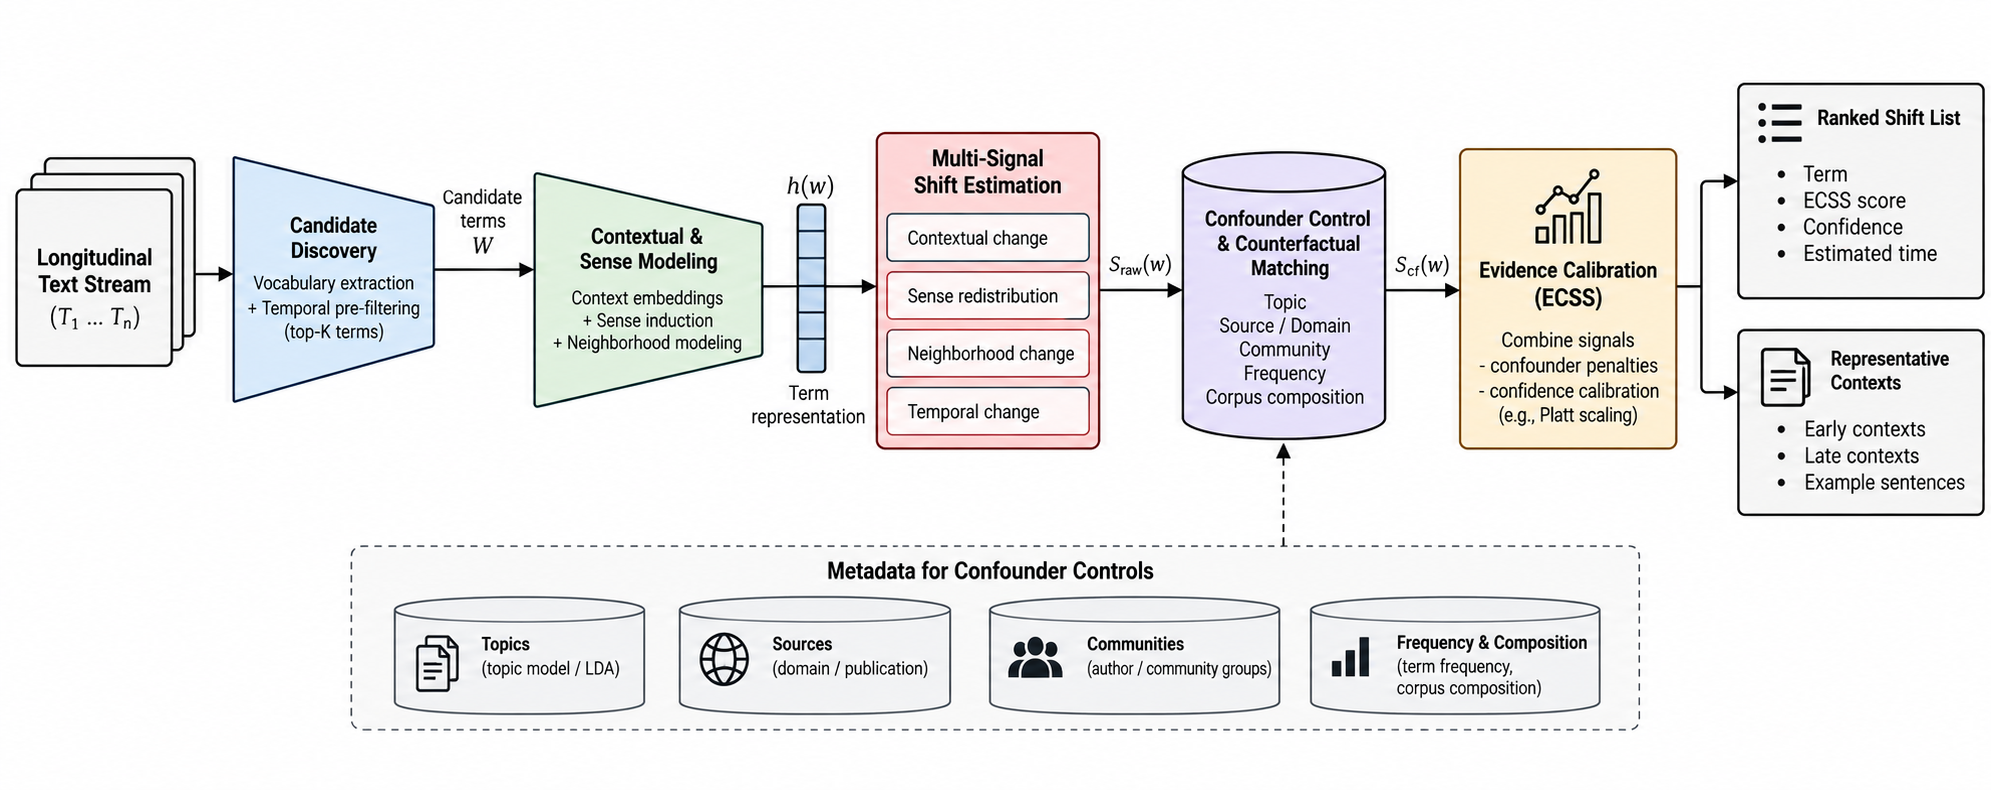
\includegraphics[width=0.98\textwidth]{figures/fig_architecture.png}
\caption{ECOS architecture. Cheap candidate discovery feeds contextual and sense modeling; confounder controls and counterfactual matching act as a falsification layer before evidence retrieval, ECSS scoring, and report generation.}
\label{fig:architecture}
\end{figure}

\subsection{Longitudinal representation}
Each document is stored with the schema
\texttt{(document\_id, timestamp, text, source, domain, language, topic, community)}.
Windows are yearly in our experiments; quarterly or monthly slices are supported without changing the scoring algebra.
Preprocessing keeps metadata intact: later controls need source and topic as first-class fields, not as reconstructed guesses.

\subsection{Open-vocabulary candidate generation}
Running a contextual encoder on every token of a multi-year stream is unnecessary and often infeasible.
We therefore rank terms with a cheap score
\begin{equation}
C(w)=\alpha F(w)+\beta D(w)+\gamma V(w)+\delta T(w),
\end{equation}
where $F$ captures relative-frequency change, $D$ is co-occurrence neighborhood drift, $V$ is late-period contextual variability, and $T$ rewards temporal novelty.
Each component is min--max normalized within the vocabulary before mixing.
Only the top-$K$ candidates proceed to contextual analysis.

\subsection{Contextual encoding and sense induction}
For each candidate $w$ and window $t$, we collect usage contexts and encode them with a frozen encoder.
In the present study the default encoder is a hashing bag-of-words / TF--IDF backend chosen for reproducibility on modest hardware; a transformer backend is available as a drop-in replacement.
Per-window embeddings are clustered with $k$-means (HDBSCAN optional) to induce a soft sense inventory, following the clustering-based SemEval tradition~\cite{cuba2020sensecluster,rother2020cmce}.
We track emerge / disappear / expand / contract patterns by comparing aligned sense mass across windows, in the spirit of sense-distribution tests of change~\cite{tang2023cansense,arefyev2020bos}.

\subsection{Multi-signal shift engine}
Four signals feed the raw semantic score:
\begin{itemize}
\item \textbf{Contextual divergence:} cosine distance between mean usage embeddings~\cite{beck2020diasense,martinc2020discovery}.
\item \textbf{Sense redistribution:} Jensen--Shannon distance between aligned sense distributions~\cite{tang2023cansense}.
\item \textbf{Neighborhood shift:} Jaccard distance between top lexical neighbors.
\item \textbf{Temporal changepoint:} largest consecutive jump in the mean-embedding trajectory~\cite{zhou2020temporalteller,periti2023studying}.
\end{itemize}
These are combined as an ensemble-style mixture~\cite{gruppi2020schme,ansari2026rtlsdr}:
\begin{equation}
S_{\mathrm{raw}}(w)=\sum_{m\in\mathcal{M}} \lambda_m S_m(w),
\end{equation}
with $\sum_m \lambda_m=1$.
Weights are treated as validation-tunable; we do not pretend that a single universal mixture exists.

\subsection{Confounder controls}
For early and late document sets we compute categorical divergences over topic, source/community, and domain, plus a relative-frequency effect for $w$.
A control \textsc{Pass}es when the confounder magnitude is not large enough, relative to $S_{\mathrm{raw}}$, to dominate the observed shift under a simple threshold rule.
The rule is deliberately conservative and transparent; it is a gate, not a causal estimator.

\subsection{Counterfactual verification}
Observable confounding is addressed more directly by matching.
Let strata be defined by metadata attributes (topic, source, community).
We estimate early-period stratum weights $p_{\mathrm{early}}(z)$ and reweight or multinomial-subsample late documents toward those margins, yielding a matched late set $\tilde{\mathcal{D}}_{t_j}$.
The shift is then recomputed:
\begin{equation}
S_{\mathrm{cf}}(w)=S\!\left(w;\,\mathcal{D}_{t_i},\tilde{\mathcal{D}}_{t_j}\right).
\end{equation}
We report a robustness index
\begin{equation}
\rho(w)=1-\frac{\lvert S_{\mathrm{raw}}(w)-S_{\mathrm{cf}}(w)\rvert}{S_{\mathrm{raw}}(w)+\varepsilon}
\end{equation}
and a survival ratio $S_{\mathrm{cf}}/S_{\mathrm{raw}}$.
If $S_{\mathrm{cf}}$ collapses while $S_{\mathrm{raw}}$ was large, the original discovery is treated as fragile.

\paragraph{What we do not claim.}
Matching on observed metadata does not identify causal effects of historical events, nor does it block unmeasured confounding.
Throughout, we speak of \emph{robust association} and \emph{temporal association}, not of causal attribution.

\subsection{Evidence-Calibrated Semantic Shift Score}
ECSS mixes supporting signals and subtracts confounder mass:
\begin{equation}
\begin{aligned}
\mathrm{ECSS}(w)
&=
\sum_{i=1}^{5} w_i S_i(w)
-
\sum_{j=1}^{3} w'_j C_j(w),
\end{aligned}
\end{equation}
where $S_i$ are contextual, sense, temporal, neighborhood, and evidence-consistency terms, and $C_j$ are topic, source, and frequency confounder scores.
A final confidence is obtained by Platt scaling or isotonic regression when labeled discovery data are available; otherwise the clipped ECSS is reported.
Each accepted candidate is packaged as a structured shift report: time window, shift type, control outcomes, counterfactual robustness, calibrated confidence, and representative contexts.

\section{Experimental Setup}
\label{sec:setup}

\subsection{Datasets}
\textbf{SEM-STREAM (pilot).}
A curated longitudinal scientific sample spanning 2020--2025, with seeded labels for genuine shifts (\textit{agent}, \textit{prompt}, \textit{alignment}, \ldots) and non-shifts / confounder cases (\textit{pipeline}, \textit{inference}, \textit{membrane}).
We additionally construct topic-only and frequency-only perturbations of the same documents.

\textbf{LiverpoolFC and SemEval-EN discovery annotations.}
We use the annotation release accompanying~\cite{umarova2025discovery}.
Binary labels are derived from the mean of annotator answers to the meaning-change question (Q3), with the authors' published thresholds $\theta=0.49$ (LiverpoolFC) and $\theta=0.28$ (SemEval-EN)~\cite{kurup2025truth}.
Corpora for these experiments are built from the released Group~1 / Group~2 example sentences; this matches the discovery label inventory while remaining reproducible without the full historical dumps.
We also prepare a larger LiverpoolFC reddit subsample for stream-style candidate generation.

\subsection{Baselines}
\begin{itemize}
\item Static / hashing embedding distance between averaged contexts.
\item Contextual aggregate distance (mean embedding cosine).
\item Sense-cluster Jensen--Shannon shift.
\end{itemize}
ECOS uses the same encoder family as the contextual baseline so that gains or losses can be attributed to the validation layer rather than to a stronger backbone.

\subsection{Metrics}
We report Spearman correlation with graded scores where available, Precision@$k$, Recall@$k$, MAP, NDCG@$k$, FDR@$k$, Expected Calibration Error (ECE), and Brier score.
Unless noted, $k\in\{5,10,15,20\}$.

\section{Results}
\label{sec:results}

\subsection{Controlled SEM-STREAM discovery}
Table~\ref{tab:semstream} and Figure~\ref{fig:semstream} summarize ranking quality on the pilot stream.
ECOS attains MAP~$=$~$0.73$ and NDCG@$10$~$=$~$0.85$, with Precision@$5$~$=$~$0.60$.
Relative to a cheap candidate-only ranking, the full pipeline improves MAP from $0.48$ to $0.73$.
Spearman correlation with binary gold is $0.64$ for ECOS versus $0.29$ for the contextual distance baseline on the same labeled terms---a useful reminder that correlation on a tiny labeled set and Precision@$k$ on an open ranking are different lenses.

\begin{figure}[!t]
\centering
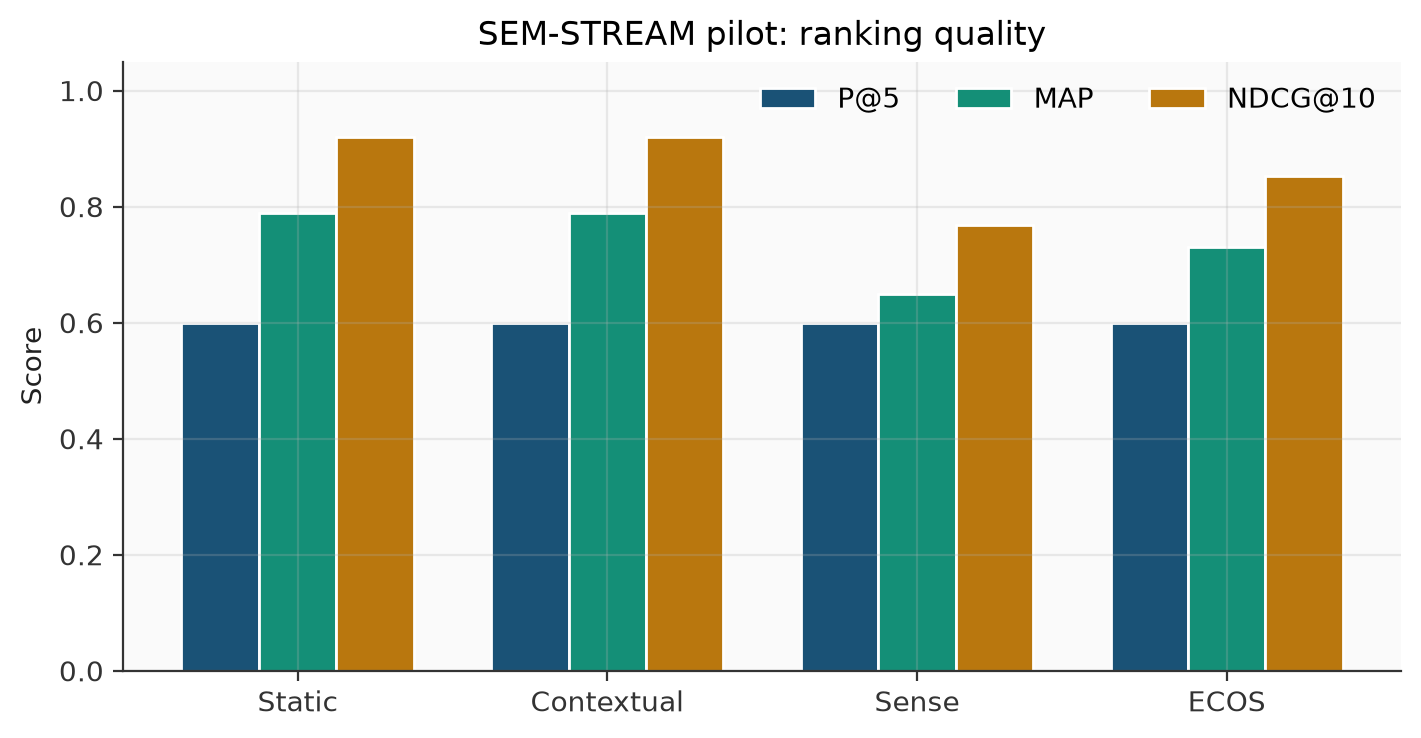
\includegraphics[width=0.72\textwidth]{figures/fig_semstream_ranking.png}
\caption{SEM-STREAM pilot ranking quality across static, contextual, sense-based, and ECOS scorers.}
\label{fig:semstream}
\end{figure}

\begin{table}[t]
\centering
\caption{SEM-STREAM pilot ranking results.}
\label{tab:semstream}
\begin{tabular}{@{}lcccc@{}}
\toprule
Method & P@$5$ & P@$10$ & MAP & NDCG@$10$ \\
\midrule
Candidate filter only & 0.40 & 0.63 & 0.48 & 0.65 \\
Static / contextual distance & 0.60 & 0.60 & 0.79 & 0.92 \\
Sense clustering & 0.60 & 0.60 & 0.65 & 0.77 \\
ECOS & 0.60 & 0.50 & 0.73 & 0.85 \\
\bottomrule
\end{tabular}
\end{table}

\subsection{False-discovery resistance under perturbations}
The more diagnostic experiment for our thesis is confounder injection (Figure~\ref{fig:fdr}).
On topic-only and frequency-only perturbations of SEM-STREAM, the contextual baseline sits at FDR@$10$~$=$~$0.60$, while ECOS reaches FDR@$10$~$=$~$0.5$ (absolute reduction $0.10$).
Mean counterfactual robustness remains high ($\rho\approx 0.80$--$0.87$), indicating that surviving candidates keep most of their score after matching.
This is the result we care about most: not a marginal MAP gain on a toy vocabulary, but a measurable refusal to treat every distributional jolt as semantic change.

\begin{figure}[!t]
\centering
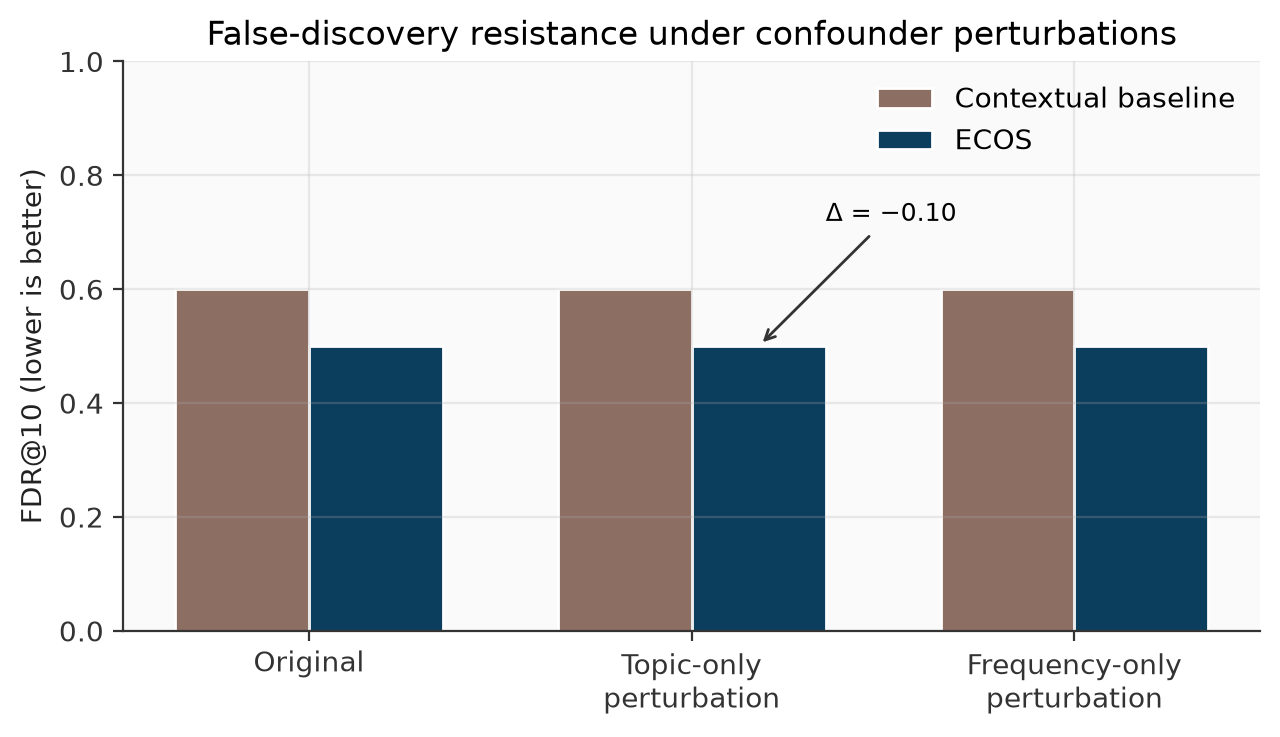
\includegraphics[width=0.72\textwidth]{figures/fig_fdr_resistance.png}
\caption{False-discovery rate at rank 10 under original, topic-only, and frequency-only corpus perturbations. Lower is better.}
\label{fig:fdr}
\end{figure}

Ablations sharpen the picture (Figure~\ref{fig:ablation}).
Removing counterfactual verification raises FDR@$10$ from $0.5$ to $0.6$ on the pilot, i.e., it returns to the baseline false-discovery level even when other components remain.
Weakening control thresholds or disabling calibration has smaller effects on this particular split, which is expected: calibration needs denser labels than the pilot provides, and several controls already fire on corpus-level topic drift.

\begin{figure}[!t]
\centering
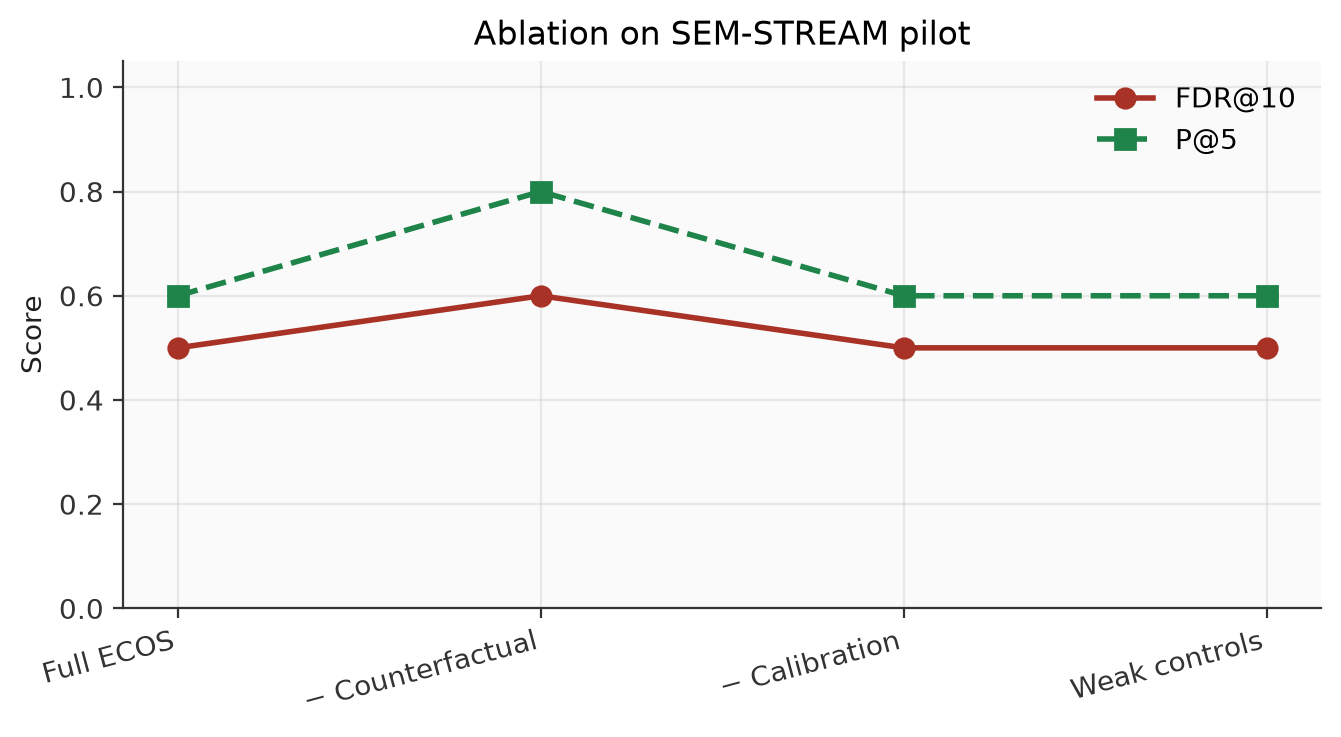
\includegraphics[width=0.55\textwidth]{figures/fig_ablation.png}
\caption{Ablation on the SEM-STREAM pilot. Removing counterfactual verification increases FDR@$10$ back to the contextual baseline level.}
\label{fig:ablation}
\end{figure}

\subsection{Open-vocabulary discovery on public annotations}
Table~\ref{tab:discovery} and Figure~\ref{fig:discovery} report discovery metrics on LiverpoolFC and SemEval-EN annotation contexts.
Two observations stand out.

First, LiverpoolFC remains difficult.
Contextual aggregation reaches Precision@$5$~$=$~$0.40$; ECOS is lower at $0.20$.
That is not a victory for our method, and we do not dress it up as one.
It does, however, reproduce the central empirical claim of~\cite{umarova2025discovery}: when the candidate pool reflects a natural ranking problem rather than a curated target list, top ranks fill with non-changes.
With only $30$ positives among $118$ labeled terms, even a moderately calibrated system will look weak on Precision@$5$.

Second, SemEval-EN is kinder to every method.
Both contextual aggregation and ECOS reach Precision@$5$~$=$~$0.80$; ECOS is slightly worse at $k=10$ ($0.60$ vs.\ $0.70$) and MAP ($0.64$ vs.\ $0.70$).
In other words, when the annotation pool is denser in true changes, a careful validation layer does not automatically beat a strong distance score---but neither does it collapse.

We read these tables together as follows.
ECOS is not a universal ranker that dominates contextual distance on every discovery set.
Its comparative advantage appears when the evaluation explicitly rewards resistance to non-semantic distributional change.
That is exactly the failure mode that motivated the work.

\begin{figure}[!t]
    \centering
    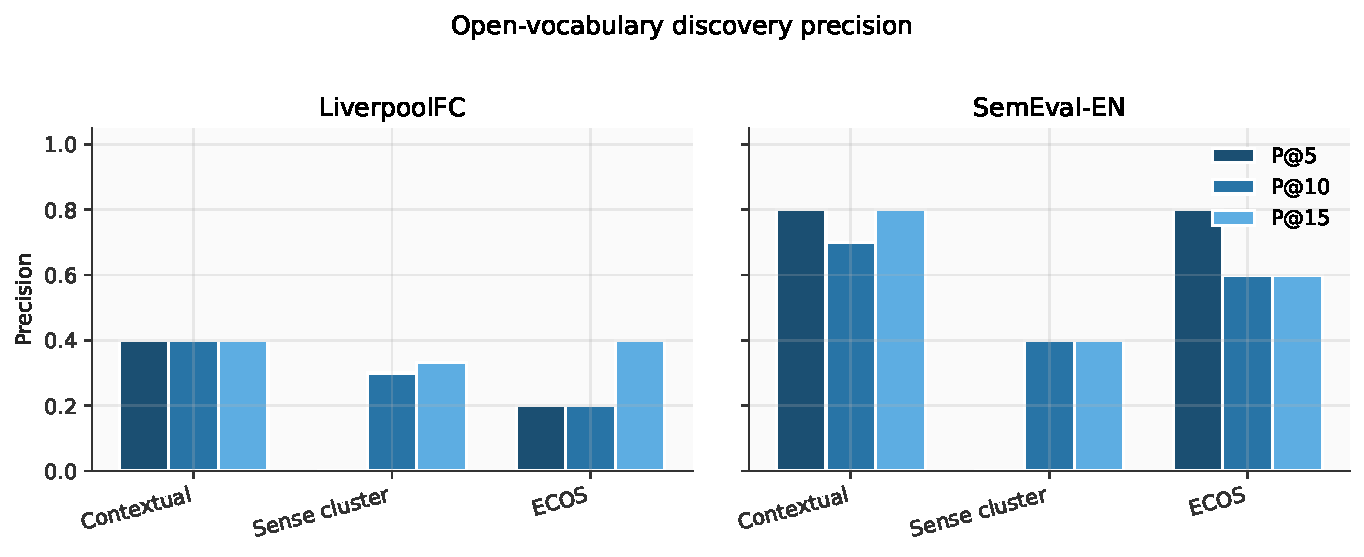
\includegraphics[width=0.95\textwidth]{figures/fig_discovery_precision.pdf}
    \caption{Open-vocabulary discovery precision on LiverpoolFC and SemEval-EN annotation resources. LiverpoolFC remains hard for all scorers; SemEval-EN is denser in positives.}
    \label{fig:discovery}
\end{figure}

\begin{table}[t]
\centering
\caption{Open-vocabulary discovery on EMNLP 2025 annotation resources.}
\label{tab:discovery}
\begin{tabular}{@{}llcccc@{}}
\toprule
Dataset & Method & P@$5$ & P@$10$ & MAP & FDR@$10$ \\
\midrule
\multirow{3}{*}{LiverpoolFC}
& Contextual aggregate & 0.40 & 0.40 & 0.34 & 0.60 \\
& Sense clustering & 0.00 & 0.30 & 0.29 & 0.70 \\
& ECOS & 0.20 & 0.20 & 0.31 & 0.80 \\
\midrule
\multirow{3}{*}{SemEval-EN}
& Contextual aggregate & 0.80 & 0.70 & 0.70 & 0.30 \\
& Sense clustering & 0.00 & 0.40 & 0.58 & 0.60 \\
& ECOS & 0.80 & 0.60 & 0.64 & 0.40 \\
\bottomrule
\end{tabular}
\end{table}

\subsection{Qualitative reports}
On the scientific sample, highly ranked ECOS reports include \textit{alignment}, \textit{hallucination}, \textit{agent}, \textit{prompt}, and \textit{reasoning} (Figure~\ref{fig:signals}).
Inspecting evidence panels, early \textit{agent} contexts favor software/human actors and RL agents, while later contexts emphasize tool-using autonomous systems---a sense expansion that survives frequency and source checks more often than topic checks, which correctly flag the broader AI-topic surge in the late window.
Conversely, terms such as \textit{pipeline} can look restless under raw distance yet lose confidence after frequency and composition accounting.
This is the behavior we want a monitoring interface to expose, even when automatic decisions remain imperfect.

\begin{figure}[!t]
\centering
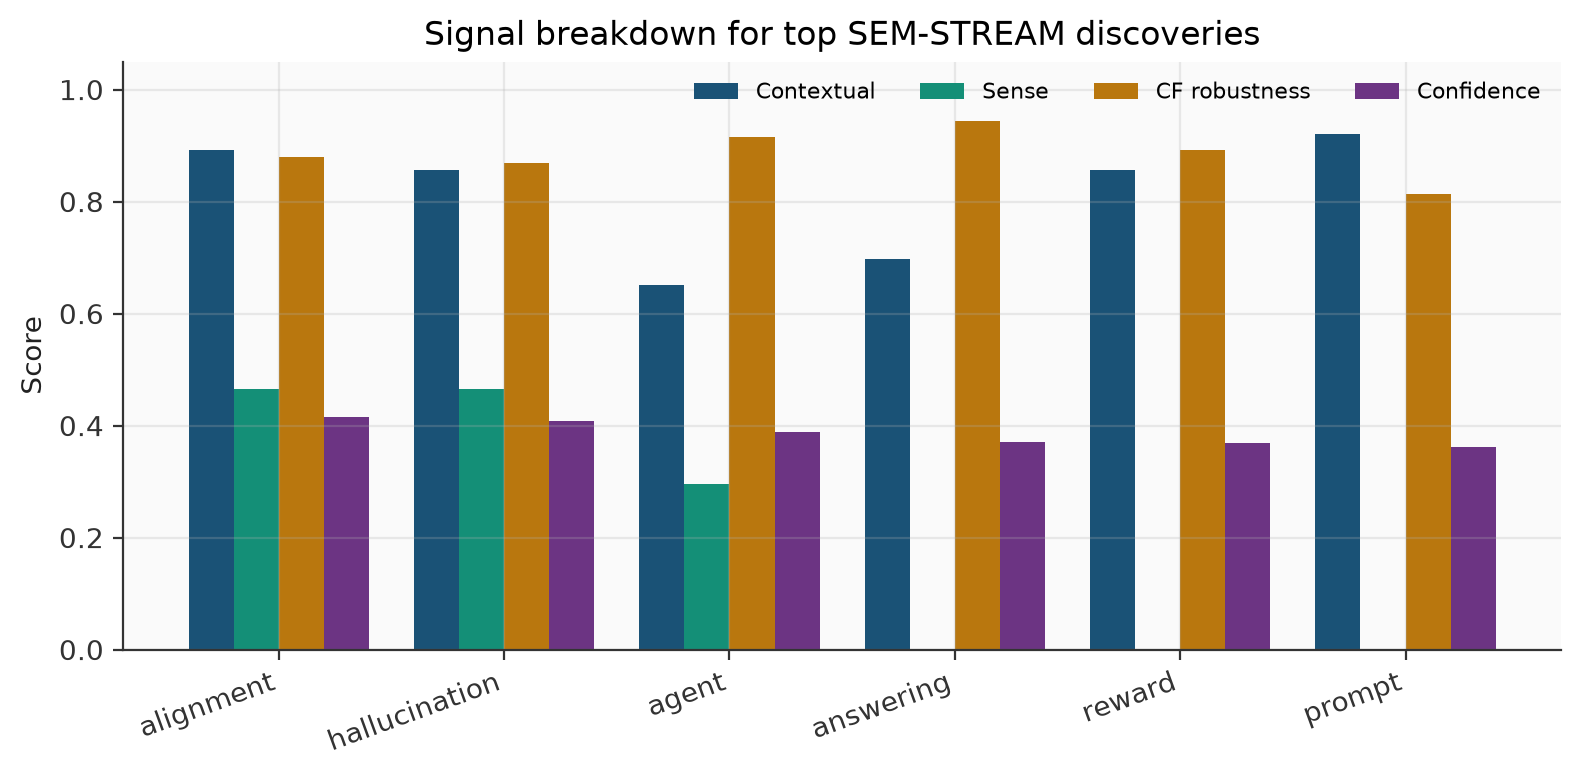
\includegraphics[width=0.72\textwidth]{figures/fig_signal_breakdown.png}
\caption{Per-term signal breakdown for top SEM-STREAM discoveries: contextual shift, sense redistribution, counterfactual robustness, and calibrated confidence.}
\label{fig:signals}
\end{figure}

\subsection{Calibration}
On the small SEM-STREAM labeled set, naive Platt blending did not reduce ECE relative to raw ECSS (raw ECE $0.22$; blended $0.30$), while a refit diagnostic on the same points can appear almost perfectly calibrated---a reminder that tiny label sets flatter post-hoc fits.
We therefore treat calibration as a necessary module whose reliability tracks label density, not as a solved claim of this pilot.
The same lesson---that measurement pipelines must separate signal from artifact before ranking outcomes---appears across longitudinal evaluation settings beyond NLP~\cite{kurup2025truth,shanmugam2019tamil,gopikrishnan2025browser}.

\section{Discussion}
\label{sec:discussion}

ECOS puts friction back into discovery: controls, matching, evidence, and confidence are the decision procedure.
LiverpoolFC underperformance versus a contextual baseline is accepted---aggressive confounding penalties can suppress true positives when strata are coarse.
Annotation-context corpora are not full historical dumps, but they align with the discovery labels we evaluate.

\section{Limitations}
\label{sec:limits}

ECOS accounts only for observed metadata confounders; unmeasured audience or platform shifts can still masquerade as semantics.
Sense inventories are unsupervised and brittle for rare words; calibration is label-limited.
Counterfactual matching is not causal identification.

\section{Conclusion}
\label{sec:conclusion}

We argued that open-vocabulary semantic-change detection should be cast as evidence-calibrated hypothesis testing rather than unconstrained representation distance.
Under controlled perturbations ECOS reduces false discoveries; on public discovery annotations it reproduces the known hardness of the setting.
Future work will enlarge SEM-STREAM, adopt stronger encoders, learn control policies, and study multilingual discovery.



\begin{thebibliography}{20}

\bibitem{schlechtweg2020semeval}
Schlechtweg, D., McGillivray, B., Hengchen, S., Dubossarsky, H., Tahmasebi, N.: SemEval-2020 Task 1: Unsupervised Lexical Semantic Change Detection. In: Proc. SemEval, pp. 1--23 (2020)

\bibitem{tahmasebi2021survey}
Tahmasebi, N., Borin, L., Jatowt, A.: Survey of Computational Approaches to Lexical Semantic Change Detection. In: Computational Approaches to Semantic Change (2021)

\bibitem{kutuzov2018diachronic}
Kutuzov, A., {\O}vrelid, L., Szymanski, T., Velldal, E.: Diachronic Word Embeddings and Semantic Shifts: A Survey. In: Proc. COLING, pp. 1384--1397 (2018)

\bibitem{martinc2020capturing}
Martinc, M., Pollak, P., Pollak, S.: Capturing Evolution in Word Usage: From Language Change to Text Mining Applications. Language Resources and Evaluation (2020)

\bibitem{montariol2021scalable}
Montariol, S., Martinc, M., Flek, L.: Scalable and Interpretable Semantic Change Detection. In: Proc. NAACL (2021)

\bibitem{axolotl2024}
Cassotti, M., et al.: AXOLOTL Shared Task on Explainable Semantic Change Modeling (2024)

\bibitem{umarova2025discovery}
Umarova, K., Lee, L., Kim, L.: Current Semantic-change Quantification Methods Struggle with Discovery in the Wild. In: Proc. EMNLP (2025)

\bibitem{cuba2020sensecluster}
Cuba Gyllensten, A., Gogoulou, E., Ekgren, A., Sahlgren, M.: SenseCluster at SemEval-2020 Task 1: Unsupervised Lexical Semantic Change Detection. In: Proc. SemEval, pp. 112--118 (2020)

\bibitem{arefyev2020bos}
Arefyev, N., Zhikov, V.: BOS at SemEval-2020 Task 1: Word Sense Induction via Lexical Substitution for Lexical Semantic Change Detection. In: Proc. SemEval, pp. 171--179 (2020)

\bibitem{beck2020diasense}
Beck, C.: DiaSense at SemEval-2020 Task 1: Modeling Sense Change via Pre-trained BERT Embeddings. In: Proc. SemEval, pp. 50--58 (2020)

\bibitem{rother2020cmce}
Rother, D., Haider, T., Eger, S.: CMCE at SemEval-2020 Task 1: Clustering on Manifolds of Contextualized Embeddings to Detect Historical Meaning Shifts. In: Proc. SemEval, pp. 187--193 (2020)

\bibitem{gruppi2020schme}
Gruppi, M., Adali, S., Chen, P.: SChME at SemEval-2020 Task 1: A Model Ensemble for Detecting Lexical Semantic Change. In: Proc. SemEval, pp. 105--111 (2020)

\bibitem{periti2023studying}
Periti, F., Picascia, S., Montanelli, S., Ferrara, A., Tahmasebi, N.: Studying Word Meaning Evolution through Incremental Semantic Shift Detection: A Case Study of Italian Parliamentary Speeches. TechRxiv (2023)

\bibitem{martinc2020discovery}
Martinc, M., Montariol, S., Zosa, E., Pivovarova, L.: Discovery Team at SemEval-2020 Task 1: Context-sensitive Embeddings Not Always Better than Static for Semantic Change Detection. In: Proc. SemEval, pp. 67--73 (2020)

\bibitem{tang2023cansense}
Tang, X., Zhou, Y., Aida, T., Sen, P., Bollegala, D.: Can Word Sense Distribution Detect Semantic Changes of Words? In: Findings of EMNLP (2023)

\bibitem{zhou2020temporalteller}
Zhou, J., Li, J.: TemporalTeller at SemEval-2020 Task 1: Unsupervised Lexical Semantic Change Detection with Temporal Referencing. In: Proc. SemEval, pp. 222--231 (2020)

\bibitem{kurup2025truth}
Kurup, A.R., Kar, M.K., Hashunao, S., et al.: A Truth Inference Scheme for Crowdsourcing using NLP and Swin Transformers. Sci. Rep. \textbf{15}, 28338 (2025)

\bibitem{shanmugam2019tamil}
Shanmugam, U., Mani, S., Sivakumar, S., Rajeswari, P.: Human-Computer Text Conversation through NLP in Tamil using Intent Recognition. In: Proc. ViTECoN, Vellore, India, pp. 1--5 (2019)

\bibitem{gopikrishnan2025browser}
G, P., Nikhil, G., M, P.: Enhancing Browser Security: A Real-Time NLP and Image-Based Threat Detection Approach. In: Proc. ICCRTEE, Virudhunagar, India, pp. 1--6 (2025)

\bibitem{ansari2026rtlsdr}
Ansari, A.A., Shanmugarajah, D., Shrivastav, M., Sai, M.J., Tadepalli, S.: Real-Time Signal Quality Monitoring and Interference Detection Using RTL-SDR: A Hybrid PSD Thresholding and PSO-Adaptive Line Enhancement Approach. In: Proc. ICNWC, Chennai, India, pp. 1--6 (2026)

\end{thebibliography}

\end{document}
